% TODO: add `final` to hide todonotes
%\documentclass[11pt,a4paper,oneside]{report}             % Single-side
\documentclass[11pt,a4paper,twoside,openright,final]{report}  % Duplex

% thanks to http://tex.stackexchange.com/a/47579/71109
\usepackage{ifxetex}
\usepackage{ifluatex}
\newif\ifxetexorluatex % a new conditional starts as false
\ifnum 0\ifxetex 1\fi\ifluatex 1\fi>0
   \xetexorluatextrue
\fi

\ifxetexorluatex
  \usepackage{fontspec}
\else
  \usepackage[T1]{fontenc}
  \usepackage[utf8]{inputenc}
  \usepackage[lighttt]{lmodern}
  \ttfamily\DeclareFontShape{T1}{lmtt}{m}{it}{<->sub*lmtt/m/sl}{}
\fi

\usepackage[english,magyar]{babel} % Alapértelmezés szerint utoljára definiált nyelv lesz aktív, de később külön beállítjuk az aktív nyelvet.

\usepackage{emptypage} % omit page number on empty pages

%\usepackage{cmap}
\usepackage{amsfonts,amsmath,amssymb} % Mathematical symbols.
%\usepackage[ruled,boxed,resetcount,linesnumbered]{algorithm2e} % For pseudocodes. % beware: this is not compatible with LuaLaTeX, see http://tex.stackexchange.com/questions/34814/lualatex-and-algorithm2e
\usepackage{booktabs} % For publication quality tables for LaTeX
\usepackage{graphicx}

%\usepackage{fancyhdr}
%\usepackage{lastpage}

\usepackage{geometry}
%\usepackage{sectsty}
\usepackage{setspace} % For setting line spacing

\usepackage[unicode]{hyperref} % For hyperlinks in the generated document.
\usepackage{xcolor}
\usepackage{listings} % For source code snippets.

\usepackage[amsmath,thmmarks]{ntheorem} % Theorem-like environments.

\usepackage[hang]{caption}

\singlespacing

\newcommand{\selecthungarian}{
	\selectlanguage{magyar}
	\setlength{\parindent}{2em}
	\setlength{\parskip}{0em}
	\frenchspacing
}

\newcommand{\selectenglish}{
	\selectlanguage{english}
	\setlength{\parindent}{0em}
	\setlength{\parskip}{0.5em}
	\nonfrenchspacing
	\renewcommand{\figureautorefname}{Figure}
	\renewcommand{\tableautorefname}{Table}
	\renewcommand{\partautorefname}{Part}
	\renewcommand{\chapterautorefname}{Chapter}
	\renewcommand{\sectionautorefname}{Section}
	\renewcommand{\subsectionautorefname}{Section}
	\renewcommand{\subsubsectionautorefname}{Section}
}

\usepackage[numbers]{natbib}
\usepackage{xspace}

\usepackage[obeyFinal]{todonotes}
\definecolor{lightblue}{rgb}{0.68, 0.85, 0.9}
\newcommand{\marci}[1]{\todo[color=lightblue]{\textbf{M:} #1}}
\newcommand{\marciLine}[1]{\todo[inline,color=lightblue]{#1}}

\usepackage{forest}
\usepackage{subfiles}


\newcommand{\vikszerzoVezeteknev}{Tieger}
\newcommand{\vikszerzoKeresztnev}{Balázs}

\newcommand{\vikkonzulensAMegszolitas}{}
\newcommand{\vikkonzulensAVezeteknev}{Elekes}
\newcommand{\vikkonzulensAKeresztnev}{Márton}

\newcommand{\vikkonzulensBMegszolitas}{}
\newcommand{\vikkonzulensBVezeteknev}{Szatmári}
\newcommand{\vikkonzulensBKeresztnev}{Zoltán}

\newcommand{\vikkonzulensCMegszolitas}{}
\newcommand{\vikkonzulensCVezeteknev}{}
\newcommand{\vikkonzulensCKeresztnev}{}

\newcommand{\vikcim}{Enforcing Kubernetes constraints using high level Dsl} % Cím
\newcommand{\viktanszek}{\bmemit} % Tanszék
\newcommand{\vikdoktipus}{\msc} % Dokumentum típusa (\bsc vagy \msc)
\newcommand{\vikmunkatipusat}{diplomatervet} % a "hallgató nyilatkozat" részhez: szakdolgozatot vagy diplomatervet


\newcommand{\szerzoMeta}{\vikszerzoVezeteknev{} \vikszerzoKeresztnev} % egy szerző esetén
%\newcommand{\szerzoMeta}{\vikszerzoVezeteknev{} \vikszerzoKeresztnev, \tdkszerzoB} % két szerző esetén


% Beállítások magyar nyelvű dolgozathoz
%%--------------------------------------------------------------------------------------
% Elnevezések
%--------------------------------------------------------------------------------------
\newcommand{\bme}{Budapesti Műszaki és Gazdaságtudományi Egyetem}
\newcommand{\vik}{Villamosmérnöki és Informatikai Kar}

\newcommand{\bmemit}{Méréstechnika és Információs Rendszerek Tanszék}

\newcommand{\keszitette}{Készítette}
\newcommand{\konzulens}{Konzulens}

\newcommand{\bsc}{Szakdolgozat}
\newcommand{\msc}{Diplomaterv}
\newcommand{\tdk}{TDK dolgozat}
\newcommand{\bsconlab}{BSc Önálló laboratórium}
\newcommand{\msconlabi}{MSc Önálló laboratórium 1.}
\newcommand{\msconlabii}{MSc Önálló laboratórium 2.}

\newcommand{\pelda}{Példa}
\newcommand{\definicio}{Definíció}
\newcommand{\tetel}{Tétel}

\newcommand{\bevezetes}{Bevezetés}
\newcommand{\koszonetnyilvanitas}{Köszönetnyilvánítás}
\newcommand{\fuggelek}{Függelék}

% Opcionálisan átnevezhető címek
%\addto\captionsmagyar{%
%\renewcommand{\listfigurename}{Saját ábrajegyzék cím}
%\renewcommand{\listtablename}{Saját táblázatjegyzék cím}
%\renewcommand{\bibname}{Saját irodalomjegyzék név}
%}

\newcommand{\szerzo}{\vikszerzoVezeteknev{} \vikszerzoKeresztnev}
\newcommand{\vikkonzulensA}{\vikkonzulensAMegszolitas\vikkonzulensAVezeteknev{} \vikkonzulensAKeresztnev}
\newcommand{\vikkonzulensB}{\vikkonzulensBMegszolitas\vikkonzulensBVezeteknev{} \vikkonzulensBKeresztnev}
\newcommand{\vikkonzulensC}{\vikkonzulensCMegszolitas\vikkonzulensCVezeteknev{} \vikkonzulensCKeresztnev}

\newcommand{\selectthesislanguage}{\selecthungarian}

\bibliographystyle{huplain}

\def\lstlistingname{kódrészlet}

\newcommand{\appendixnumber}{6}  % a fofejezet-szamlalo az angol ABC 6. betuje (F) lesz

%--------------------------------------------------------------------------------------
% Elnevezések
%--------------------------------------------------------------------------------------
\newcommand{\bme}{Budapest University of Technology and Economics}
\newcommand{\vik}{Faculty of Electrical Engineering and Informatics}

\newcommand{\bmemit}{Department of Measurement and Information Systems}

\newcommand{\keszitette}{Author}
\newcommand{\konzulens}{Advisor}

\newcommand{\bsc}{Bachelor's Thesis}
\newcommand{\msc}{Master's Thesis}
\newcommand{\tdk}{Scientific Students' Association Report}
\newcommand{\bsconlab}{BSc Project Laboratory}
\newcommand{\msconlabi}{MSc Project Laboratory 1}
\newcommand{\msconlabii}{MSc Project Laboratory 2}

\newcommand{\pelda}{Example}
\newcommand{\definicio}{Definition}
\newcommand{\tetel}{Theorem}

\newcommand{\bevezetes}{Introduction}
\newcommand{\koszonetnyilvanitas}{Acknowledgements}
\newcommand{\fuggelek}{Appendix}

% Optional custom titles
%\addto\captionsenglish{%
%\renewcommand*{\listfigurename}{Your list of figures title}
%\renewcommand*{\listtablename}{Your list of tables title}
%\renewcommand*{\bibname}{Your bibliography title}
%}

\newcommand{\szerzo}{\vikszerzoKeresztnev{} \vikszerzoVezeteknev}
\newcommand{\vikkonzulensA}{\vikkonzulensAMegszolitas\vikkonzulensAKeresztnev{} \vikkonzulensAVezeteknev}
\newcommand{\vikkonzulensB}{\vikkonzulensBMegszolitas\vikkonzulensBKeresztnev{} \vikkonzulensBVezeteknev}
\newcommand{\vikkonzulensC}{\vikkonzulensCMegszolitas\vikkonzulensCKeresztnev{} \vikkonzulensCVezeteknev}

\newcommand{\selectthesislanguage}{\selectenglish}

\bibliographystyle{plainnat}

\newcommand{\ie}{i.e.\@\xspace}
\newcommand{\Ie}{I.e.\@\xspace}
\newcommand{\eg}{e.g.\@\xspace}
\newcommand{\Eg}{E.g.\@\xspace}
\newcommand{\etal}{et al.\@\xspace}
\newcommand{\etc}{etc.\@\xspace}
\newcommand{\vs}{vs.\@\xspace}
\newcommand{\viz}{viz.\@\xspace} % videlicet
\newcommand{\cf}{cf.\@\xspace} % confer
\newcommand{\Cf}{Cf.\@\xspace}
\newcommand{\wrt}{w.r.t.\@\xspace} % with respect to
\newcommand{\approximately}{approx.\@\xspace}

\newcommand{\appendixnumber}{1}  % a fofejezet-szamlalo az angol ABC 1. betuje (A) lesz


%--------------------------------------------------------------------------------------
% Page layout setup
%--------------------------------------------------------------------------------------
% we need to redefine the pagestyle plain
% another possibility is to use the body of this command without \fancypagestyle
% and use \pagestyle{fancy} but in that case the special pages
% (like the ToC, the References, and the Chapter pages)remain in plane style

\pagestyle{plain}
\geometry{inner=35mm, outer=25mm, top=28mm, bottom=25mm}

\setcounter{tocdepth}{3}
%\sectionfont{\large\upshape\bfseries}
\setcounter{secnumdepth}{3}

\sloppy % Margón túllógó sorok tiltása.
\widowpenalty=10000 \clubpenalty=10000 %A fattyú- és árvasorok elkerülése
\def\hyph{-\penalty0\hskip0pt\relax} % Kötőjeles szavak elválasztásának engedélyezése


%--------------------------------------------------------------------------------------
% Setup hyperref package
%--------------------------------------------------------------------------------------
\hypersetup{
    % bookmarks=true,            % show bookmarks bar?
    unicode=true,              % non-Latin characters in Acrobat's bookmarks
    pdftitle={\vikcim},        % title
    pdfauthor={\szerzoMeta},    % author
    pdfsubject={\vikdoktipus}, % subject of the document
    pdfcreator={\szerzoMeta},   % creator of the document
    pdfproducer={},    % producer of the document
    pdfkeywords={},    % list of keywords (separate then by comma)
    pdfnewwindow=true,         % links in new window
    colorlinks=true,           % false: boxed links; true: colored links
    linkcolor=black,           % color of internal links
    citecolor=black,           % color of links to bibliography
    filecolor=black,           % color of file links
    urlcolor=black             % color of external links
}


% https://www.overleaf.com/learn/latex/Code_listing

\definecolor{commentsColor}{rgb}{0.1, 0.7, 0.1}
\definecolor{numberingcolor}{rgb}{0.497495, 0.497587, 0.497464}
\definecolor{keywordsColor}{rgb}{0.000000, 0.000000, 0.635294}
\definecolor{stringColor}{rgb}{0.6, 0.05, 0.15}

% \usepackage{fontspec}
% \newfontfamily{\ttconsolas}{Consolas}[Scale=0.8]
\lstset{ %
  backgroundcolor=\color{white},   % choose the background color; you must add \usepackage{color} or \usepackage{xcolor}
  %basicstyle=\ttfamily,        % the size of the fonts that are used for the code
  basicstyle=\ttfamily\footnotesize,
  breakatwhitespace=false,         % sets if automatic breaks should only happen at whitespace
  breaklines=true,                 % sets automatic line breaking
  captionpos=b,                    % sets the caption-position to bottom
  commentstyle=\color{commentsColor}\textit,    % comment style
  deletekeywords={...},            % if you want to delete keywords from the given language
  escapeinside={\%*}{*)},          % if you want to add LaTeX within your code
  extendedchars=true,              % lets you use non-ASCII characters; for 8-bits encodings only, does not work with UTF-8
  frame=tb,	                   	   % adds a frame around the code
  keepspaces=true,                 % keeps spaces in text, useful for keeping indentation of code (possibly needs columns=flexible)
  keywordstyle=\color{keywordsColor}\bfseries,       % keyword style
  language=Java,                   % the language of the code (can be overrided per snippet)
  numbers=left,                    % where to put the line-numbers; possible values are (none, left, right)
  numbersep=5pt,                   % how far the line-numbers are from the code
  numberstyle=\tiny\color{numberingcolor}, % the style that is used for the line-numbers
  rulecolor=\color{black},         % if not set, the frame-color may be changed on line-breaks within not-black text (e.g. comments (green here))
  showspaces=false,                % show spaces everywhere adding particular underscores; it overrides 'showstringspaces'
  showstringspaces=false,          % underline spaces within strings only
  showtabs=false,                  % show tabs within strings adding particular underscores
  stepnumber=1,                    % the step between two line-numbers. If it's 1, each line will be numbered
  stringstyle=\color{stringColor}, % string literal style
  tabsize=2,	                   % sets default tabsize to 2 spaces
  title=\lstname,                  % show the filename of files included with \lstinputlisting; also try caption instead of title
  columns=fixed                    % Using fixed column width (for e.g. nice alignment)
}



\lstdefinelanguage{Java11}{
  morekeywords={var, void, public, private, new, final, class, protected, abstract, static, import, package, return, boolean, synchronized, if, else, throws, int, throw, null, try, catch, for, while},
  sensitive=true, % keywords are not case-sensitive
  morecomment=[l]{//}, % l is for line comment
  morecomment=[s]{/*}{*/}, % s is for start and end delimiter
  morestring=[b]" % defines that strings are enclosed in double quotes
}

\lstdefinelanguage{MySQL}{
  morekeywords={INSERT, IGNORE, INTO, VALUES},
  sensitive=true, % keywords are not case-sensitive
  morestring=[b]' % defines that strings are enclosed in double quotes
}

\lstdefinelanguage{Kotlin}{
  morekeywords={fun, class, object, var, val, if, else, internal, return, private, by, data, annotation, typealias, infix},
  sensitive=true, % keywords are not case-sensitive
  morecomment=[l]{//}, % l is for line comment
  morecomment=[s]{/*}{*/}, % s is for start and end delimiter
  morestring=[b]" % defines that strings are enclosed in double quotes
}

\lstdefinelanguage{JSON}{
  morekeywords={null, true, false},
  sensitive=true, % keywords are not case-sensitive
  morecomment=[l]{//}, % l is for line comment
  morecomment=[s]{/*}{*/}, % s is for start and end delimiter
  morestring=[b]" % defines that strings are enclosed in double quotes
}

\lstdefinelanguage{YAML}{
  morekeywords={null, true, false},
  sensitive=true, % keywords are not case-sensitive
  morecomment=[l]{\#}, % l is for line comment
  morestring=[b]" % defines that strings are enclosed in double quotes
}

%--------------------------------------------------------------------------------------
% Set up theorem-like environments
%--------------------------------------------------------------------------------------
% Using ntheorem package -- see http://www.math.washington.edu/tex-archive/macros/latex/contrib/ntheorem/ntheorem.pdf

\theoremstyle{plain}
\theoremseparator{.}
\newtheorem{example}{\pelda}

\theoremseparator{.}
%\theoremprework{\bigskip\hrule\medskip}
%\theorempostwork{\hrule\bigskip}
\theorembodyfont{\upshape}
\theoremsymbol{{\large \ensuremath{\centerdot}}}
\newtheorem{definition}{\definicio}

\theoremseparator{.}
%\theoremprework{\bigskip\hrule\medskip}
%\theorempostwork{\hrule\bigskip}
\newtheorem{theorem}{\tetel}


%--------------------------------------------------------------------------------------
% Some new commands and declarations
%--------------------------------------------------------------------------------------
\newcommand{\code}[1]{{\upshape\ttfamily\scriptsize\indent #1}}
\newcommand{\doi}[1]{DOI: \href{http://dx.doi.org/\detokenize{#1}}{\raggedright{\texttt{\detokenize{#1}}}}} % A hivatkozások közt így könnyebb DOI-t megadni.

\DeclareMathOperator*{\argmax}{arg\,max}
%\DeclareMathOperator*[1]{\floor}{arg\,max}
\DeclareMathOperator{\sign}{sgn}
\DeclareMathOperator{\rot}{rot}


%--------------------------------------------------------------------------------------
% Setup captions
%--------------------------------------------------------------------------------------
\captionsetup[figure]{aboveskip=10pt}

\renewcommand{\captionlabelfont}{\bf}
%\renewcommand{\captionfont}{\footnotesize\it}

%--------------------------------------------------------------------------------------
% Hyphenation exceptions
%--------------------------------------------------------------------------------------
\hyphenation{Shakes-peare Mar-seilles ár-víz-tű-rő tü-kör-fú-ró-gép}


\author{\vikszerzo}
\title{\viktitle}


%--------------------------------------------------------------------------------------
% Table of contents and the main text
%--------------------------------------------------------------------------------------
\begin{document}

\pagenumbering{gobble}


\selectthesislanguage


%~~~~~~~~~~~~~~~~~~~~~~~~~~~~~~~~~~~~~~~~~~~~~~~~~~~~~~~~~~~~~~~~~~~~~~~~~~~~~~~~~~~~~~
\hypersetup{pageanchor=false}
%--------------------------------------------------------------------------------------
%	The title page
%--------------------------------------------------------------------------------------
\begin{titlepage}
\begin{center}

\includegraphics[width=60mm,keepaspectratio]{figures/bme_logo.pdf}\\
\vspace{0.3cm}
\textbf{\bme}\\
\textmd{\vik}\\
\textmd{\viktanszek}\\[5cm]

\vspace{0.4cm}
{\huge \bfseries \vikcim}\\[0.8cm]
\vspace{0.5cm}
\textsc{\Large \vikdoktipus}\\[4cm]

{
	\renewcommand{\arraystretch}{0.85}
	\begin{tabular}{cc}
	 \makebox[7cm]{\emph{\keszitette}} & \makebox[7cm]{\emph{\konzulens}} \\ \noalign{\smallskip}
	 \makebox[7cm]{\szerzo} & \makebox[7cm]{\vikkonzulensA} \\
	  & \makebox[7cm]{\vikkonzulensB} \\
	  & \makebox[7cm]{\vikkonzulensC} \\
	\end{tabular}
}

%\todo[inline]{Add final to \textbackslash documentclass in thesis.tex to hide todos; check that there are no remaining todos (and \textbackslash listoftodos) by commenting \textbackslash usepackage ... todonotes out in packages.tex}

\vfill
{\large \today}
\end{center}
\end{titlepage}
\hypersetup{pageanchor=false}

		   % Szakdolgozat/Diplomaterv címlap

%\listoftodos

% Table of Contents
%~~~~~~~~~~~~~~~~~~~~~~~~~~~~~~~~~~~~~~~~~~~~~~~~~~~~~~~~~~~~~~~~~~~~~~~~~~~~~~~~~~~~~~
\setcounter{tocdepth}{1}
\tableofcontents\cleardoublepage


% Declaration and Abstract
%~~~~~~~~~~~~~~~~~~~~~~~~~~~~~~~~~~~~~~~~~~~~~~~~~~~~~~~~~~~~~~~~~~~~~~~~~~~~~~~~~~~~~~
% \selectlanguage{magyar}
\pagenumbering{gobble}
%--------------------------------------------------------------------------------------
% Nyilatkozat
%--------------------------------------------------------------------------------------
\begin{center}
\large
\textbf{HALLGATÓI NYILATKOZAT}\\
\end{center}

Alulírott \emph{\vikszerzoVezeteknev{} \vikszerzoKeresztnev}, szigorló hallgató kijelentem, hogy ezt a \vikmunkatipusat{} meg nem engedett segítség nélkül, saját magam készítettem, csak a megadott forrásokat (szakirodalom, eszközök stb.) használtam fel. Minden olyan részt, melyet szó szerint, vagy azonos értelemben, de átfogalmazva más forrásból átvettem, egyértelműen, a forrás megadásával megjelöltem.

Hozzájárulok, hogy a jelen munkám alapadatait (szerző(k), cím, angol és magyar nyelvű tartalmi kivonat, készítés éve, konzulens(ek) neve) a BME VIK nyilvánosan hozzáférhető elektronikus formában, a munka teljes szövegét pedig az egyetem belső hálózatán keresztül (vagy autentikált felhasználók számára) közzétegye. Kijelentem, hogy a benyújtott munka és annak elektronikus verziója megegyezik. Dékáni engedéllyel titkosított diplomatervek esetén a dolgozat szövege csak 3 év eltelte után válik hozzáférhetővé.

\begin{flushleft}
\vspace*{1cm}
Budapest, \today
\end{flushleft}

\begin{flushright}
 \vspace*{1cm}
 \makebox[7cm]{\rule{6cm}{.4pt}}\\
 \makebox[7cm]{\emph{\vikszerzoVezeteknev{} \vikszerzoKeresztnev}}\\
 \makebox[7cm]{hallgató}
\end{flushright}
\thispagestyle{empty}

\vfill
\cleardoublepage

\selectthesislanguage

\pagenumbering{roman}
\setcounter{page}{1}

\selecthungarian

\setlength{\parindent}{0pt}
\setlength{\parskip}{0.6em}

%----------------------------------------------------------------------------
% Abstract in Hungarian
%----------------------------------------------------------------------------
\chapter*{Kivonat}\addcontentsline{toc}{chapter}{Kivonat}

Manapság az alkalmazásfejlesztés fő trendje a rendszer több komponensre bontása és ezeknek a komponenseknek konténerekbe csomagolása, valamint harmadik féltől származó megoldásokkal való integrálása. Az ilyen több komponensű elosztott alkalmazások tipikus üzemeltetési környezete a Kubernetes, amely rugalmas megoldást kínál ebben a témakörben felmerülő legtöbb problémára.

Egy Kubernetesre írt alkalmazás megfelelő üzemeltetése nagy kihívás az elosztott rendszerek üzemeltetéséből eredő komplexitás miatt. Egy működőképes rendszer összeállítása nem mindig elegendő. Éppen ezért a megfelelő működésen felül lehetnek nem funkcionális követelmények is a rendszerrel szemben, például rendelkezésre állási vagy biztonsági követelmények. Az ilyen követelmények betartatása nem triviális.

Dolgozatom célja egy kényszerek leírását lehetővé tevő szakterület-specifikus nyelv megalkotása és egy kényszerek betartatását segítő keretrendszer kialakítása, amely keretrendszer jelentősen megkönnyíti a Kubernetes alapú rendszerekben nem funkcionális követelmények betartatását és ellenőrzését.

Az elkészített nyelv egy Kotlin DSL, ami a Kotlin programozási nyelvhez készült szoftverkönyvtárat jelenti. A nyelven kívül a keretrendszer része egy fordító a nyelvhez, egy kényszereket futtató ágens és egy menedzser komponens, ami felügyeli az ágenseket, és intézi a telepítésüket és konfigurálásukat.

Az általam megtervezett és megvalósított keretrendszer lehetőséget ad kényszerek megsértésének detektálására, valamint olyan új események megvétózására vagy módosítására, amik megsértenének bizonyos kényszereket. Továbbá összeállítottam egy csokor Kubernetes világában bevált gyakorlatot (best practice), és a nyelv segítségével leírtam azokat. Az elkészült rendszert és bevált gyakorlatokat demonstráltam egy élethű esettanulmányon keresztül.

\vfill
\selectenglish


%----------------------------------------------------------------------------
% Abstract in English
%----------------------------------------------------------------------------
\chapter*{Abstract}\addcontentsline{toc}{chapter}{Abstract}

These days, the main trend in application development is to split the system into several components and package these components in containers and integrate them with third-party solutions. A typical operating environment for such multi-component distributed applications is Kubernetes, which offers a flexible solution to most of the problems that arise in this field.

The proper operation of an application written on Kubernetes is a big challenge due to the complexity resulting from the operation of distributed systems. Putting together a workable system is not always enough. That is why, in addition to proper operation, there may also be non-functional requirements for the system, such as availability or security requirements. Compliance with such requirements is not trivial.

The objective of my thesis is to develop a domain-specific language that enables the description of constraints and create a framework that facilitates the enforcement of these constraints, significantly easing compliance and control of non-functional requirements in Kubernetes-based systems.

The created language is a Kotlin DSL, which is essentially a software library for the Kotlin programming language. In addition to the language, the framework includes a compiler for the language, an agent that runs the constraints, and a manager component that oversees the agents and manages their installation and configuration.

The framework I designed and implemented provides the capability to detect violations of constraints, as well as to veto or modify new events that would violate certain constraints. Furthermore, I collected a set of Kubernetes best practices and implemented them using my language. I demonstrated the implemented system and set of best practices through a true-to-life case study.

\vfill
\cleardoublepage

\selectthesislanguage

\newcounter{romanPage}
\setcounter{romanPage}{\value{page}}
\stepcounter{romanPage}


% The main part of the thesis
%~~~~~~~~~~~~~~~~~~~~~~~~~~~~~~~~~~~~~~~~~~~~~~~~~~~~~~~~~~~~~~~~~~~~~~~~~~~~~~~~~~~~~~
\pagenumbering{arabic}

%~~~~~~~~~~~~~~~~~~~~~~~~~~~~~~~~~~~~~~~~~~~~~~~~~~~~~~~~~~~~~~~~~~~~~~~~~~~~~~~~~~~~~~
% My content
%~~~~~~~~~~~~~~~~~~~~~~~~~~~~~~~~~~~~~~~~~~~~~~~~~~~~~~~~~~~~~~~~~~~~~~~~~~~~~~~~~~~~~~

\chapter{Case study 2: Creating new constraints}
\label{chap:case_study2}

The \ref{chap:case_study1} chapter only showed the capabilities of the Konstrainer framework, but did not show how to write a more advanced script, because the \nameref{chap:konst_dsl} chapter was a prerequisite for that. This chapter will continue the case study.

\section{Writing your own policies}

Let's assume the company has introduced some custom policies and, now they want to enforce them using Konstrainer. Start with a very simple policy: All images must come from the internal company registry.

To enforce this, first let's detect which pods violate this policy:

Create a file with the company-policies.kt file with the following content:

\begin{lstlisting}[caption={Report skeleton},language=Kotlin,label=code:todo]
package me.btieger

import me.btieger.dsl.*

const val companyPrefix = "tiegris/"
val companPolicies = server("company-policies") {
  report {

  }
}
\end{lstlisting}

This script has an empty report so far. As described in the \ref{sec:report} section, we should fetch the list of pods and create an aggregation group. In this case, no additional processing is needed.

\begin{lstlisting}[caption={Aggregation group},language=Kotlin,label=code:todo]
report {
  val pods = kubelist { pods() }
  aggregation("Pods", pods) {

  }
}
\end{lstlisting}

To decide if all the containers of a pod are using images only from the company registry, we must specify this requirement with mathematical precision, using first order logic. Here are two continuous sentences which, express the requirement with first order logic.

`Tag the pod, if any of its containers image does not start with the company prefix.'

`Do not tag the pod, if all of its containers image starts with the company prefix.'

\begin{lstlisting}[caption={Tag pods},language=Kotlin,label=code:todo]
report {
  aggregation("Pods", kubelist { pods() }) {
    tag("Image not from company registry") {
      item.spec.containers.any { !it.image.startsWith(companyPrefix) }
    }
  }
}
\end{lstlisting}

The script accesses the Kubernetes API, but to do that successfully, it needs authorization. We need to associate a \emph{ClusterRole} to the agent. In the demo files there is also a \emph{ClusterRole} definition. We want our agent to be least privileged, so we are only giving it read access to the pods.

\begin{lstlisting}[caption={TODO},language=Kotlin,label=code:todo]
package me.btieger
import me.btieger.dsl.*

const val companyPrefix = "tiegris/"
val companyPolicies = server("company-policies") {
  clusterRole = "read-pods"
  report {
    aggregation("Pods", kubelist { pods() }) {
      tag("Image not from company registry") {
        item.spec.containers.any { !it.image.startsWith(companyPrefix) }
      }
    }
  }
}
\end{lstlisting}

The line: `clusterRole = ReadAny` assigns the ReadAny clusterrole to the agent by creating a clusterrolebinding during the deployment of the agent. The ReadAny clusterrole is created with the Konstrainer installation, it gives read access to all resources in the cluster.

Let's test the script now. If we upload, and deploy the script, we should see it working:

\begin{figure}[h]
  \centering
  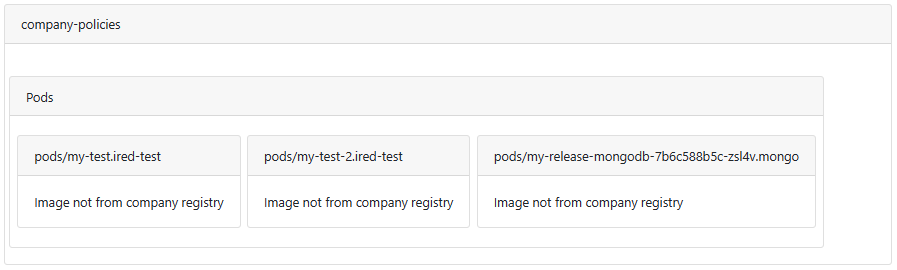
\includegraphics[width=130mm, keepaspectratio]{content/60_caseStudy2/company_policies_1.png}
  \caption{Report generated by the script}
  \label{fig:report}
\end{figure}

The report shows that there are 3 pods, which use images outside from the company registry.

Now lets do the enforcing part. Put this code inside the server block.

\begin{lstlisting}[caption={TODO},language=Kotlin,label=code:todo]
webhook("only-internal-registry") {
  operations(CREATE, UPDATE)
  apiGroups(APPS)
  apiVersions(ANY)
  resources(DEPLOYMENTS, STATEFULSETS, DAEMONSETS)
  namespaceSelector { }
  failurePolicy(FAIL)
  behavior {
    allowed {
      podSpec!!.containers.all { it.image.startsWith(companyPrefix) }
    }
    status {
      message = "All images must be from the company registry."
    }
  }
}
\end{lstlisting}

To create a rule, we need to add a `webhook` block. It needs a unique name. Lets name it "only-internal-registry". We need to define which events should the webhook listen to. In this example the webhook listens to the creation or update of any deployments, statefulsets and daemonsets.

The more interesting part is the behavior block. It describes how should the webhook behave when a request arrives. Inside the behavior block we can access the request body using many ways. One of them is the podSpec keyword. It is a shortcut to the `.spec.template.spec` of a deployment, statefulset or daemonset.

In the allowed block we can specify when to allow or reject an event. In this case we only accept events when the all the containers of the pod has an image starting with the the company prefix.

In the status block we define the error message in case the event is rejected.

Lets deploy and test our newly created agent dsl. On the monitors view we can see that the pods inside the ired-test namespace use images outside of the company registry, and the mongodb also uses an image from docker.io instead of the company registry.

We can also test that we can no longer create resources which use images outside from the company registry:

\begin{lstlisting}[caption={TODO},language=bash,label=code:bashx]
kubectl create ns policy-test
kubectl apply -f k8s/test-policy.yaml -n policy-test
\end{lstlisting}

We should get this error:

\begin{lstlisting}[caption={TODO},language=bash,label=code:todo]
Error from server: error when creating "k8s/test-policy.yaml": admission webhook "only-internal-registry.btieger.me" denied the request: All images must be from the company registry.
\end{lstlisting}

\begin{lstlisting}[caption={TODO},language=bash,label=code:bashx]
yq eval 'select(.kind == "Deployment").spec.template.spec.containers[0].image = "tiegris/apples-users"' k8s/test-policy.yaml -i
kubectl apply -f k8s/test-policy.yaml -n policy-test
\end{lstlisting}

This error shows that our rule works and is enforced.

This is the end of the demo. In this demo we saw the basic capabilities of the Konstrainer platform, some use-cases, and how to create our own rules.


\chapter{Case study 2: Creating new constraints}
\label{chap:case_study2}

The \ref{chap:case_study1} chapter only showed the capabilities of the Konstrainer framework, but did not show how to write a more advanced script, because the \nameref{chap:konst_dsl} chapter was a prerequisite for that. This chapter will continue the case study.

\section{Writing your own policies}

Let's assume the company has introduced some custom policies and, now they want to enforce them using Konstrainer. Start with a very simple policy: All images must come from the internal company registry.

To enforce this, first let's detect which pods violate this policy:

Create a file with the company-policies.kt file with the following content:

\begin{lstlisting}[caption={Report skeleton},language=Kotlin,label=code:todo]
package me.btieger

import me.btieger.dsl.*

const val companyPrefix = "tiegris/"
val companPolicies = server("company-policies") {
  report {

  }
}
\end{lstlisting}

This script has an empty report so far. As described in the \ref{sec:report} section, we should fetch the list of pods and create an aggregation group. In this case, no additional processing is needed.

\begin{lstlisting}[caption={Aggregation group},language=Kotlin,label=code:todo]
report {
  val pods = kubelist { pods() }
  aggregation("Pods", pods) {

  }
}
\end{lstlisting}

To decide if all the containers of a pod are using images only from the company registry, we must specify this requirement with mathematical precision, using first order logic. Here are two continuous sentences which, express the requirement with first order logic.

`Tag the pod, if any of its containers image does not start with the company prefix.'

`Do not tag the pod, if all of its containers image starts with the company prefix.'

\begin{lstlisting}[caption={Tag pods},language=Kotlin,label=code:todo]
report {
  aggregation("Pods", kubelist { pods() }) {
    tag("Image not from company registry") {
      item.spec.containers.any { !it.image.startsWith(companyPrefix) }
    }
  }
}
\end{lstlisting}

The script accesses the Kubernetes API, but to do that successfully, it needs authorization. We need to associate a \emph{ClusterRole} to the agent. In the demo files there is also a \emph{ClusterRole} definition. We want our agent to be least privileged, so we are only giving it read access to the pods.

\begin{lstlisting}[caption={TODO},language=Kotlin,label=code:todo]
package me.btieger
import me.btieger.dsl.*

const val companyPrefix = "tiegris/"
val companyPolicies = server("company-policies") {
  clusterRole = "read-pods"
  report {
    aggregation("Pods", kubelist { pods() }) {
      tag("Image not from company registry") {
        item.spec.containers.any { !it.image.startsWith(companyPrefix) }
      }
    }
  }
}
\end{lstlisting}

The line: `clusterRole = ReadAny` assigns the ReadAny clusterrole to the agent by creating a clusterrolebinding during the deployment of the agent. The ReadAny clusterrole is created with the Konstrainer installation, it gives read access to all resources in the cluster.

Let's test the script now. If we upload, and deploy the script, we should see it working:

\begin{figure}[h]
  \centering
  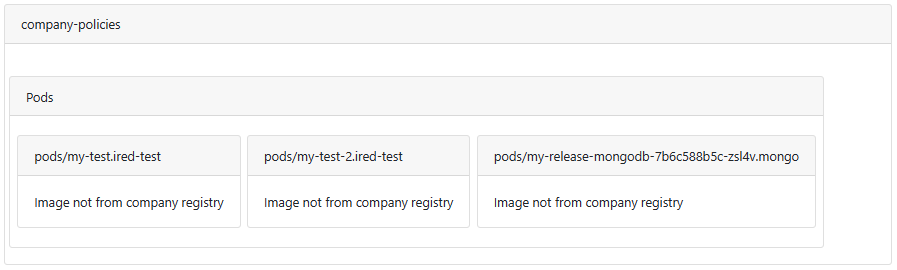
\includegraphics[width=130mm, keepaspectratio]{content/60_caseStudy2/company_policies_1.png}
  \caption{Report generated by the script}
  \label{fig:report}
\end{figure}

The report shows that there are 3 pods, which use images outside from the company registry.

Now lets do the enforcing part. Put this code inside the server block.

\begin{lstlisting}[caption={TODO},language=Kotlin,label=code:todo]
webhook("only-internal-registry") {
  operations(CREATE, UPDATE)
  apiGroups(APPS)
  apiVersions(ANY)
  resources(DEPLOYMENTS, STATEFULSETS, DAEMONSETS)
  namespaceSelector { }
  failurePolicy(FAIL)
  behavior {
    allowed {
      podSpec!!.containers.all { it.image.startsWith(companyPrefix) }
    }
    status {
      message = "All images must be from the company registry."
    }
  }
}
\end{lstlisting}

To create a rule, we need to add a `webhook` block. It needs a unique name. Lets name it "only-internal-registry". We need to define which events should the webhook listen to. In this example the webhook listens to the creation or update of any deployments, statefulsets and daemonsets.

The more interesting part is the behavior block. It describes how should the webhook behave when a request arrives. Inside the behavior block we can access the request body using many ways. One of them is the podSpec keyword. It is a shortcut to the `.spec.template.spec` of a deployment, statefulset or daemonset.

In the allowed block we can specify when to allow or reject an event. In this case we only accept events when the all the containers of the pod has an image starting with the the company prefix.

In the status block we define the error message in case the event is rejected.

Lets deploy and test our newly created agent dsl. On the monitors view we can see that the pods inside the ired-test namespace use images outside of the company registry, and the mongodb also uses an image from docker.io instead of the company registry.

We can also test that we can no longer create resources which use images outside from the company registry:

\begin{lstlisting}[caption={TODO},language=bash,label=code:bashx]
kubectl create ns policy-test
kubectl apply -f k8s/test-policy.yaml -n policy-test
\end{lstlisting}

We should get this error:

\begin{lstlisting}[caption={TODO},language=bash,label=code:todo]
Error from server: error when creating "k8s/test-policy.yaml": admission webhook "only-internal-registry.btieger.me" denied the request: All images must be from the company registry.
\end{lstlisting}

\begin{lstlisting}[caption={TODO},language=bash,label=code:bashx]
yq eval 'select(.kind == "Deployment").spec.template.spec.containers[0].image = "tiegris/apples-users"' k8s/test-policy.yaml -i
kubectl apply -f k8s/test-policy.yaml -n policy-test
\end{lstlisting}

This error shows that our rule works and is enforced.

This is the end of the demo. In this demo we saw the basic capabilities of the Konstrainer platform, some use-cases, and how to create our own rules.


\chapter{Case study 2: Creating new constraints}
\label{chap:case_study2}

The \ref{chap:case_study1} chapter only showed the capabilities of the Konstrainer framework, but did not show how to write a more advanced script, because the \nameref{chap:konst_dsl} chapter was a prerequisite for that. This chapter will continue the case study.

\section{Writing your own policies}

Let's assume the company has introduced some custom policies and, now they want to enforce them using Konstrainer. Start with a very simple policy: All images must come from the internal company registry.

To enforce this, first let's detect which pods violate this policy:

Create a file with the company-policies.kt file with the following content:

\begin{lstlisting}[caption={Report skeleton},language=Kotlin,label=code:todo]
package me.btieger

import me.btieger.dsl.*

const val companyPrefix = "tiegris/"
val companPolicies = server("company-policies") {
  report {

  }
}
\end{lstlisting}

This script has an empty report so far. As described in the \ref{sec:report} section, we should fetch the list of pods and create an aggregation group. In this case, no additional processing is needed.

\begin{lstlisting}[caption={Aggregation group},language=Kotlin,label=code:todo]
report {
  val pods = kubelist { pods() }
  aggregation("Pods", pods) {

  }
}
\end{lstlisting}

To decide if all the containers of a pod are using images only from the company registry, we must specify this requirement with mathematical precision, using first order logic. Here are two continuous sentences which, express the requirement with first order logic.

`Tag the pod, if any of its containers image does not start with the company prefix.'

`Do not tag the pod, if all of its containers image starts with the company prefix.'

\begin{lstlisting}[caption={Tag pods},language=Kotlin,label=code:todo]
report {
  aggregation("Pods", kubelist { pods() }) {
    tag("Image not from company registry") {
      item.spec.containers.any { !it.image.startsWith(companyPrefix) }
    }
  }
}
\end{lstlisting}

The script accesses the Kubernetes API, but to do that successfully, it needs authorization. We need to associate a \emph{ClusterRole} to the agent. In the demo files there is also a \emph{ClusterRole} definition. We want our agent to be least privileged, so we are only giving it read access to the pods.

\begin{lstlisting}[caption={TODO},language=Kotlin,label=code:todo]
package me.btieger
import me.btieger.dsl.*

const val companyPrefix = "tiegris/"
val companyPolicies = server("company-policies") {
  clusterRole = "read-pods"
  report {
    aggregation("Pods", kubelist { pods() }) {
      tag("Image not from company registry") {
        item.spec.containers.any { !it.image.startsWith(companyPrefix) }
      }
    }
  }
}
\end{lstlisting}

The line: `clusterRole = ReadAny` assigns the ReadAny clusterrole to the agent by creating a clusterrolebinding during the deployment of the agent. The ReadAny clusterrole is created with the Konstrainer installation, it gives read access to all resources in the cluster.

Let's test the script now. If we upload, and deploy the script, we should see it working:

\begin{figure}[h]
  \centering
  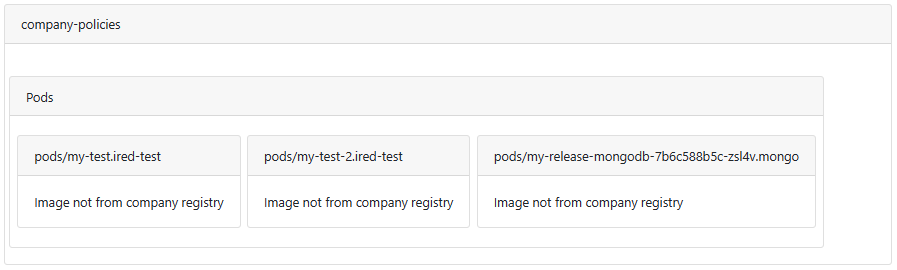
\includegraphics[width=130mm, keepaspectratio]{content/60_caseStudy2/company_policies_1.png}
  \caption{Report generated by the script}
  \label{fig:report}
\end{figure}

The report shows that there are 3 pods, which use images outside from the company registry.

Now lets do the enforcing part. Put this code inside the server block.

\begin{lstlisting}[caption={TODO},language=Kotlin,label=code:todo]
webhook("only-internal-registry") {
  operations(CREATE, UPDATE)
  apiGroups(APPS)
  apiVersions(ANY)
  resources(DEPLOYMENTS, STATEFULSETS, DAEMONSETS)
  namespaceSelector { }
  failurePolicy(FAIL)
  behavior {
    allowed {
      podSpec!!.containers.all { it.image.startsWith(companyPrefix) }
    }
    status {
      message = "All images must be from the company registry."
    }
  }
}
\end{lstlisting}

To create a rule, we need to add a `webhook` block. It needs a unique name. Lets name it "only-internal-registry". We need to define which events should the webhook listen to. In this example the webhook listens to the creation or update of any deployments, statefulsets and daemonsets.

The more interesting part is the behavior block. It describes how should the webhook behave when a request arrives. Inside the behavior block we can access the request body using many ways. One of them is the podSpec keyword. It is a shortcut to the `.spec.template.spec` of a deployment, statefulset or daemonset.

In the allowed block we can specify when to allow or reject an event. In this case we only accept events when the all the containers of the pod has an image starting with the the company prefix.

In the status block we define the error message in case the event is rejected.

Lets deploy and test our newly created agent dsl. On the monitors view we can see that the pods inside the ired-test namespace use images outside of the company registry, and the mongodb also uses an image from docker.io instead of the company registry.

We can also test that we can no longer create resources which use images outside from the company registry:

\begin{lstlisting}[caption={TODO},language=bash,label=code:bashx]
kubectl create ns policy-test
kubectl apply -f k8s/test-policy.yaml -n policy-test
\end{lstlisting}

We should get this error:

\begin{lstlisting}[caption={TODO},language=bash,label=code:todo]
Error from server: error when creating "k8s/test-policy.yaml": admission webhook "only-internal-registry.btieger.me" denied the request: All images must be from the company registry.
\end{lstlisting}

\begin{lstlisting}[caption={TODO},language=bash,label=code:bashx]
yq eval 'select(.kind == "Deployment").spec.template.spec.containers[0].image = "tiegris/apples-users"' k8s/test-policy.yaml -i
kubectl apply -f k8s/test-policy.yaml -n policy-test
\end{lstlisting}

This error shows that our rule works and is enforced.

This is the end of the demo. In this demo we saw the basic capabilities of the Konstrainer platform, some use-cases, and how to create our own rules.


\chapter{Case study 2: Creating new constraints}
\label{chap:case_study2}

The \ref{chap:case_study1} chapter only showed the capabilities of the Konstrainer framework, but did not show how to write a more advanced script, because the \nameref{chap:konst_dsl} chapter was a prerequisite for that. This chapter will continue the case study.

\section{Writing your own policies}

Let's assume the company has introduced some custom policies and, now they want to enforce them using Konstrainer. Start with a very simple policy: All images must come from the internal company registry.

To enforce this, first let's detect which pods violate this policy:

Create a file with the company-policies.kt file with the following content:

\begin{lstlisting}[caption={Report skeleton},language=Kotlin,label=code:todo]
package me.btieger

import me.btieger.dsl.*

const val companyPrefix = "tiegris/"
val companPolicies = server("company-policies") {
  report {

  }
}
\end{lstlisting}

This script has an empty report so far. As described in the \ref{sec:report} section, we should fetch the list of pods and create an aggregation group. In this case, no additional processing is needed.

\begin{lstlisting}[caption={Aggregation group},language=Kotlin,label=code:todo]
report {
  val pods = kubelist { pods() }
  aggregation("Pods", pods) {

  }
}
\end{lstlisting}

To decide if all the containers of a pod are using images only from the company registry, we must specify this requirement with mathematical precision, using first order logic. Here are two continuous sentences which, express the requirement with first order logic.

`Tag the pod, if any of its containers image does not start with the company prefix.'

`Do not tag the pod, if all of its containers image starts with the company prefix.'

\begin{lstlisting}[caption={Tag pods},language=Kotlin,label=code:todo]
report {
  aggregation("Pods", kubelist { pods() }) {
    tag("Image not from company registry") {
      item.spec.containers.any { !it.image.startsWith(companyPrefix) }
    }
  }
}
\end{lstlisting}

The script accesses the Kubernetes API, but to do that successfully, it needs authorization. We need to associate a \emph{ClusterRole} to the agent. In the demo files there is also a \emph{ClusterRole} definition. We want our agent to be least privileged, so we are only giving it read access to the pods.

\begin{lstlisting}[caption={TODO},language=Kotlin,label=code:todo]
package me.btieger
import me.btieger.dsl.*

const val companyPrefix = "tiegris/"
val companyPolicies = server("company-policies") {
  clusterRole = "read-pods"
  report {
    aggregation("Pods", kubelist { pods() }) {
      tag("Image not from company registry") {
        item.spec.containers.any { !it.image.startsWith(companyPrefix) }
      }
    }
  }
}
\end{lstlisting}

The line: `clusterRole = ReadAny` assigns the ReadAny clusterrole to the agent by creating a clusterrolebinding during the deployment of the agent. The ReadAny clusterrole is created with the Konstrainer installation, it gives read access to all resources in the cluster.

Let's test the script now. If we upload, and deploy the script, we should see it working:

\begin{figure}[h]
  \centering
  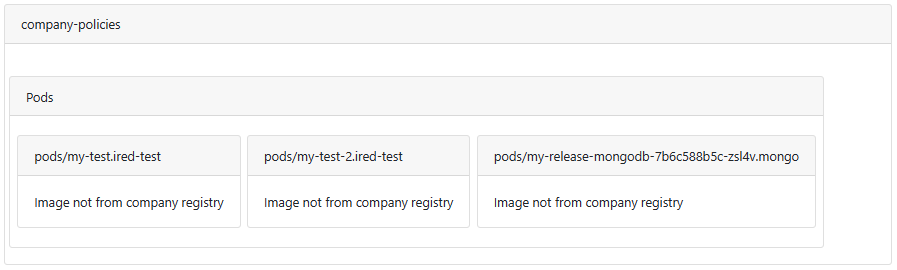
\includegraphics[width=130mm, keepaspectratio]{content/60_caseStudy2/company_policies_1.png}
  \caption{Report generated by the script}
  \label{fig:report}
\end{figure}

The report shows that there are 3 pods, which use images outside from the company registry.

Now lets do the enforcing part. Put this code inside the server block.

\begin{lstlisting}[caption={TODO},language=Kotlin,label=code:todo]
webhook("only-internal-registry") {
  operations(CREATE, UPDATE)
  apiGroups(APPS)
  apiVersions(ANY)
  resources(DEPLOYMENTS, STATEFULSETS, DAEMONSETS)
  namespaceSelector { }
  failurePolicy(FAIL)
  behavior {
    allowed {
      podSpec!!.containers.all { it.image.startsWith(companyPrefix) }
    }
    status {
      message = "All images must be from the company registry."
    }
  }
}
\end{lstlisting}

To create a rule, we need to add a `webhook` block. It needs a unique name. Lets name it "only-internal-registry". We need to define which events should the webhook listen to. In this example the webhook listens to the creation or update of any deployments, statefulsets and daemonsets.

The more interesting part is the behavior block. It describes how should the webhook behave when a request arrives. Inside the behavior block we can access the request body using many ways. One of them is the podSpec keyword. It is a shortcut to the `.spec.template.spec` of a deployment, statefulset or daemonset.

In the allowed block we can specify when to allow or reject an event. In this case we only accept events when the all the containers of the pod has an image starting with the the company prefix.

In the status block we define the error message in case the event is rejected.

Lets deploy and test our newly created agent dsl. On the monitors view we can see that the pods inside the ired-test namespace use images outside of the company registry, and the mongodb also uses an image from docker.io instead of the company registry.

We can also test that we can no longer create resources which use images outside from the company registry:

\begin{lstlisting}[caption={TODO},language=bash,label=code:bashx]
kubectl create ns policy-test
kubectl apply -f k8s/test-policy.yaml -n policy-test
\end{lstlisting}

We should get this error:

\begin{lstlisting}[caption={TODO},language=bash,label=code:todo]
Error from server: error when creating "k8s/test-policy.yaml": admission webhook "only-internal-registry.btieger.me" denied the request: All images must be from the company registry.
\end{lstlisting}

\begin{lstlisting}[caption={TODO},language=bash,label=code:bashx]
yq eval 'select(.kind == "Deployment").spec.template.spec.containers[0].image = "tiegris/apples-users"' k8s/test-policy.yaml -i
kubectl apply -f k8s/test-policy.yaml -n policy-test
\end{lstlisting}

This error shows that our rule works and is enforced.

This is the end of the demo. In this demo we saw the basic capabilities of the Konstrainer platform, some use-cases, and how to create our own rules.


\chapter{Case study 2: Creating new constraints}
\label{chap:case_study2}

The \ref{chap:case_study1} chapter only showed the capabilities of the Konstrainer framework, but did not show how to write a more advanced script, because the \nameref{chap:konst_dsl} chapter was a prerequisite for that. This chapter will continue the case study.

\section{Writing your own policies}

Let's assume the company has introduced some custom policies and, now they want to enforce them using Konstrainer. Start with a very simple policy: All images must come from the internal company registry.

To enforce this, first let's detect which pods violate this policy:

Create a file with the company-policies.kt file with the following content:

\begin{lstlisting}[caption={Report skeleton},language=Kotlin,label=code:todo]
package me.btieger

import me.btieger.dsl.*

const val companyPrefix = "tiegris/"
val companPolicies = server("company-policies") {
  report {

  }
}
\end{lstlisting}

This script has an empty report so far. As described in the \ref{sec:report} section, we should fetch the list of pods and create an aggregation group. In this case, no additional processing is needed.

\begin{lstlisting}[caption={Aggregation group},language=Kotlin,label=code:todo]
report {
  val pods = kubelist { pods() }
  aggregation("Pods", pods) {

  }
}
\end{lstlisting}

To decide if all the containers of a pod are using images only from the company registry, we must specify this requirement with mathematical precision, using first order logic. Here are two continuous sentences which, express the requirement with first order logic.

`Tag the pod, if any of its containers image does not start with the company prefix.'

`Do not tag the pod, if all of its containers image starts with the company prefix.'

\begin{lstlisting}[caption={Tag pods},language=Kotlin,label=code:todo]
report {
  aggregation("Pods", kubelist { pods() }) {
    tag("Image not from company registry") {
      item.spec.containers.any { !it.image.startsWith(companyPrefix) }
    }
  }
}
\end{lstlisting}

The script accesses the Kubernetes API, but to do that successfully, it needs authorization. We need to associate a \emph{ClusterRole} to the agent. In the demo files there is also a \emph{ClusterRole} definition. We want our agent to be least privileged, so we are only giving it read access to the pods.

\begin{lstlisting}[caption={TODO},language=Kotlin,label=code:todo]
package me.btieger
import me.btieger.dsl.*

const val companyPrefix = "tiegris/"
val companyPolicies = server("company-policies") {
  clusterRole = "read-pods"
  report {
    aggregation("Pods", kubelist { pods() }) {
      tag("Image not from company registry") {
        item.spec.containers.any { !it.image.startsWith(companyPrefix) }
      }
    }
  }
}
\end{lstlisting}

The line: `clusterRole = ReadAny` assigns the ReadAny clusterrole to the agent by creating a clusterrolebinding during the deployment of the agent. The ReadAny clusterrole is created with the Konstrainer installation, it gives read access to all resources in the cluster.

Let's test the script now. If we upload, and deploy the script, we should see it working:

\begin{figure}[h]
  \centering
  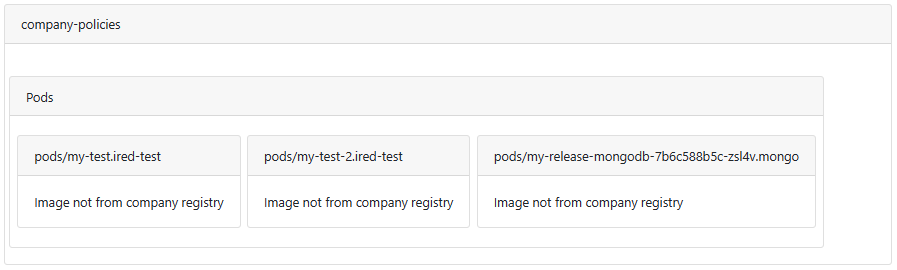
\includegraphics[width=130mm, keepaspectratio]{content/60_caseStudy2/company_policies_1.png}
  \caption{Report generated by the script}
  \label{fig:report}
\end{figure}

The report shows that there are 3 pods, which use images outside from the company registry.

Now lets do the enforcing part. Put this code inside the server block.

\begin{lstlisting}[caption={TODO},language=Kotlin,label=code:todo]
webhook("only-internal-registry") {
  operations(CREATE, UPDATE)
  apiGroups(APPS)
  apiVersions(ANY)
  resources(DEPLOYMENTS, STATEFULSETS, DAEMONSETS)
  namespaceSelector { }
  failurePolicy(FAIL)
  behavior {
    allowed {
      podSpec!!.containers.all { it.image.startsWith(companyPrefix) }
    }
    status {
      message = "All images must be from the company registry."
    }
  }
}
\end{lstlisting}

To create a rule, we need to add a `webhook` block. It needs a unique name. Lets name it "only-internal-registry". We need to define which events should the webhook listen to. In this example the webhook listens to the creation or update of any deployments, statefulsets and daemonsets.

The more interesting part is the behavior block. It describes how should the webhook behave when a request arrives. Inside the behavior block we can access the request body using many ways. One of them is the podSpec keyword. It is a shortcut to the `.spec.template.spec` of a deployment, statefulset or daemonset.

In the allowed block we can specify when to allow or reject an event. In this case we only accept events when the all the containers of the pod has an image starting with the the company prefix.

In the status block we define the error message in case the event is rejected.

Lets deploy and test our newly created agent dsl. On the monitors view we can see that the pods inside the ired-test namespace use images outside of the company registry, and the mongodb also uses an image from docker.io instead of the company registry.

We can also test that we can no longer create resources which use images outside from the company registry:

\begin{lstlisting}[caption={TODO},language=bash,label=code:bashx]
kubectl create ns policy-test
kubectl apply -f k8s/test-policy.yaml -n policy-test
\end{lstlisting}

We should get this error:

\begin{lstlisting}[caption={TODO},language=bash,label=code:todo]
Error from server: error when creating "k8s/test-policy.yaml": admission webhook "only-internal-registry.btieger.me" denied the request: All images must be from the company registry.
\end{lstlisting}

\begin{lstlisting}[caption={TODO},language=bash,label=code:bashx]
yq eval 'select(.kind == "Deployment").spec.template.spec.containers[0].image = "tiegris/apples-users"' k8s/test-policy.yaml -i
kubectl apply -f k8s/test-policy.yaml -n policy-test
\end{lstlisting}

This error shows that our rule works and is enforced.

This is the end of the demo. In this demo we saw the basic capabilities of the Konstrainer platform, some use-cases, and how to create our own rules.


\chapter{Case study 2: Creating new constraints}
\label{chap:case_study2}

The \ref{chap:case_study1} chapter only showed the capabilities of the Konstrainer framework, but did not show how to write a more advanced script, because the \nameref{chap:konst_dsl} chapter was a prerequisite for that. This chapter will continue the case study.

\section{Writing your own policies}

Let's assume the company has introduced some custom policies and, now they want to enforce them using Konstrainer. Start with a very simple policy: All images must come from the internal company registry.

To enforce this, first let's detect which pods violate this policy:

Create a file with the company-policies.kt file with the following content:

\begin{lstlisting}[caption={Report skeleton},language=Kotlin,label=code:todo]
package me.btieger

import me.btieger.dsl.*

const val companyPrefix = "tiegris/"
val companPolicies = server("company-policies") {
  report {

  }
}
\end{lstlisting}

This script has an empty report so far. As described in the \ref{sec:report} section, we should fetch the list of pods and create an aggregation group. In this case, no additional processing is needed.

\begin{lstlisting}[caption={Aggregation group},language=Kotlin,label=code:todo]
report {
  val pods = kubelist { pods() }
  aggregation("Pods", pods) {

  }
}
\end{lstlisting}

To decide if all the containers of a pod are using images only from the company registry, we must specify this requirement with mathematical precision, using first order logic. Here are two continuous sentences which, express the requirement with first order logic.

`Tag the pod, if any of its containers image does not start with the company prefix.'

`Do not tag the pod, if all of its containers image starts with the company prefix.'

\begin{lstlisting}[caption={Tag pods},language=Kotlin,label=code:todo]
report {
  aggregation("Pods", kubelist { pods() }) {
    tag("Image not from company registry") {
      item.spec.containers.any { !it.image.startsWith(companyPrefix) }
    }
  }
}
\end{lstlisting}

The script accesses the Kubernetes API, but to do that successfully, it needs authorization. We need to associate a \emph{ClusterRole} to the agent. In the demo files there is also a \emph{ClusterRole} definition. We want our agent to be least privileged, so we are only giving it read access to the pods.

\begin{lstlisting}[caption={TODO},language=Kotlin,label=code:todo]
package me.btieger
import me.btieger.dsl.*

const val companyPrefix = "tiegris/"
val companyPolicies = server("company-policies") {
  clusterRole = "read-pods"
  report {
    aggregation("Pods", kubelist { pods() }) {
      tag("Image not from company registry") {
        item.spec.containers.any { !it.image.startsWith(companyPrefix) }
      }
    }
  }
}
\end{lstlisting}

The line: `clusterRole = ReadAny` assigns the ReadAny clusterrole to the agent by creating a clusterrolebinding during the deployment of the agent. The ReadAny clusterrole is created with the Konstrainer installation, it gives read access to all resources in the cluster.

Let's test the script now. If we upload, and deploy the script, we should see it working:

\begin{figure}[h]
  \centering
  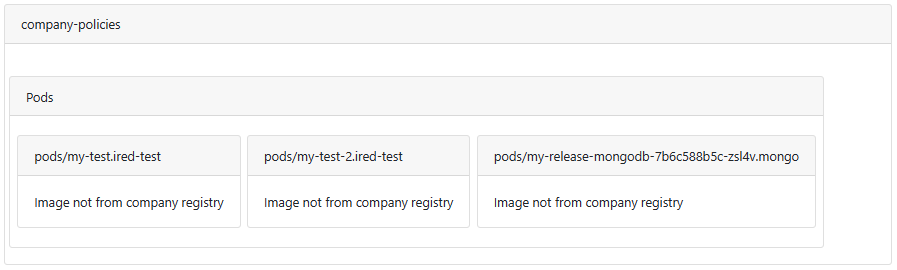
\includegraphics[width=130mm, keepaspectratio]{content/60_caseStudy2/company_policies_1.png}
  \caption{Report generated by the script}
  \label{fig:report}
\end{figure}

The report shows that there are 3 pods, which use images outside from the company registry.

Now lets do the enforcing part. Put this code inside the server block.

\begin{lstlisting}[caption={TODO},language=Kotlin,label=code:todo]
webhook("only-internal-registry") {
  operations(CREATE, UPDATE)
  apiGroups(APPS)
  apiVersions(ANY)
  resources(DEPLOYMENTS, STATEFULSETS, DAEMONSETS)
  namespaceSelector { }
  failurePolicy(FAIL)
  behavior {
    allowed {
      podSpec!!.containers.all { it.image.startsWith(companyPrefix) }
    }
    status {
      message = "All images must be from the company registry."
    }
  }
}
\end{lstlisting}

To create a rule, we need to add a `webhook` block. It needs a unique name. Lets name it "only-internal-registry". We need to define which events should the webhook listen to. In this example the webhook listens to the creation or update of any deployments, statefulsets and daemonsets.

The more interesting part is the behavior block. It describes how should the webhook behave when a request arrives. Inside the behavior block we can access the request body using many ways. One of them is the podSpec keyword. It is a shortcut to the `.spec.template.spec` of a deployment, statefulset or daemonset.

In the allowed block we can specify when to allow or reject an event. In this case we only accept events when the all the containers of the pod has an image starting with the the company prefix.

In the status block we define the error message in case the event is rejected.

Lets deploy and test our newly created agent dsl. On the monitors view we can see that the pods inside the ired-test namespace use images outside of the company registry, and the mongodb also uses an image from docker.io instead of the company registry.

We can also test that we can no longer create resources which use images outside from the company registry:

\begin{lstlisting}[caption={TODO},language=bash,label=code:bashx]
kubectl create ns policy-test
kubectl apply -f k8s/test-policy.yaml -n policy-test
\end{lstlisting}

We should get this error:

\begin{lstlisting}[caption={TODO},language=bash,label=code:todo]
Error from server: error when creating "k8s/test-policy.yaml": admission webhook "only-internal-registry.btieger.me" denied the request: All images must be from the company registry.
\end{lstlisting}

\begin{lstlisting}[caption={TODO},language=bash,label=code:bashx]
yq eval 'select(.kind == "Deployment").spec.template.spec.containers[0].image = "tiegris/apples-users"' k8s/test-policy.yaml -i
kubectl apply -f k8s/test-policy.yaml -n policy-test
\end{lstlisting}

This error shows that our rule works and is enforced.

This is the end of the demo. In this demo we saw the basic capabilities of the Konstrainer platform, some use-cases, and how to create our own rules.


\chapter{Case study 2: Creating new constraints}
\label{chap:case_study2}

The \ref{chap:case_study1} chapter only showed the capabilities of the Konstrainer framework, but did not show how to write a more advanced script, because the \nameref{chap:konst_dsl} chapter was a prerequisite for that. This chapter will continue the case study.

\section{Writing your own policies}

Let's assume the company has introduced some custom policies and, now they want to enforce them using Konstrainer. Start with a very simple policy: All images must come from the internal company registry.

To enforce this, first let's detect which pods violate this policy:

Create a file with the company-policies.kt file with the following content:

\begin{lstlisting}[caption={Report skeleton},language=Kotlin,label=code:todo]
package me.btieger

import me.btieger.dsl.*

const val companyPrefix = "tiegris/"
val companPolicies = server("company-policies") {
  report {

  }
}
\end{lstlisting}

This script has an empty report so far. As described in the \ref{sec:report} section, we should fetch the list of pods and create an aggregation group. In this case, no additional processing is needed.

\begin{lstlisting}[caption={Aggregation group},language=Kotlin,label=code:todo]
report {
  val pods = kubelist { pods() }
  aggregation("Pods", pods) {

  }
}
\end{lstlisting}

To decide if all the containers of a pod are using images only from the company registry, we must specify this requirement with mathematical precision, using first order logic. Here are two continuous sentences which, express the requirement with first order logic.

`Tag the pod, if any of its containers image does not start with the company prefix.'

`Do not tag the pod, if all of its containers image starts with the company prefix.'

\begin{lstlisting}[caption={Tag pods},language=Kotlin,label=code:todo]
report {
  aggregation("Pods", kubelist { pods() }) {
    tag("Image not from company registry") {
      item.spec.containers.any { !it.image.startsWith(companyPrefix) }
    }
  }
}
\end{lstlisting}

The script accesses the Kubernetes API, but to do that successfully, it needs authorization. We need to associate a \emph{ClusterRole} to the agent. In the demo files there is also a \emph{ClusterRole} definition. We want our agent to be least privileged, so we are only giving it read access to the pods.

\begin{lstlisting}[caption={TODO},language=Kotlin,label=code:todo]
package me.btieger
import me.btieger.dsl.*

const val companyPrefix = "tiegris/"
val companyPolicies = server("company-policies") {
  clusterRole = "read-pods"
  report {
    aggregation("Pods", kubelist { pods() }) {
      tag("Image not from company registry") {
        item.spec.containers.any { !it.image.startsWith(companyPrefix) }
      }
    }
  }
}
\end{lstlisting}

The line: `clusterRole = ReadAny` assigns the ReadAny clusterrole to the agent by creating a clusterrolebinding during the deployment of the agent. The ReadAny clusterrole is created with the Konstrainer installation, it gives read access to all resources in the cluster.

Let's test the script now. If we upload, and deploy the script, we should see it working:

\begin{figure}[h]
  \centering
  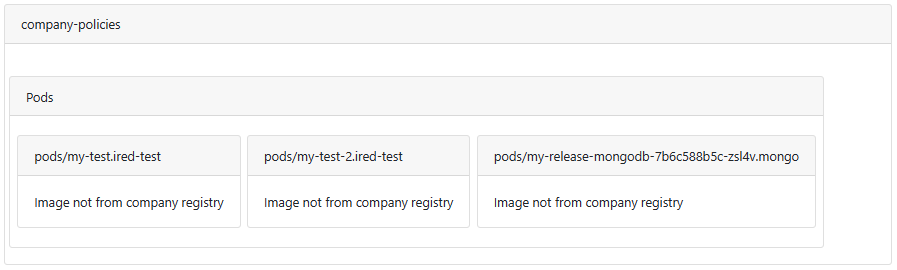
\includegraphics[width=130mm, keepaspectratio]{content/60_caseStudy2/company_policies_1.png}
  \caption{Report generated by the script}
  \label{fig:report}
\end{figure}

The report shows that there are 3 pods, which use images outside from the company registry.

Now lets do the enforcing part. Put this code inside the server block.

\begin{lstlisting}[caption={TODO},language=Kotlin,label=code:todo]
webhook("only-internal-registry") {
  operations(CREATE, UPDATE)
  apiGroups(APPS)
  apiVersions(ANY)
  resources(DEPLOYMENTS, STATEFULSETS, DAEMONSETS)
  namespaceSelector { }
  failurePolicy(FAIL)
  behavior {
    allowed {
      podSpec!!.containers.all { it.image.startsWith(companyPrefix) }
    }
    status {
      message = "All images must be from the company registry."
    }
  }
}
\end{lstlisting}

To create a rule, we need to add a `webhook` block. It needs a unique name. Lets name it "only-internal-registry". We need to define which events should the webhook listen to. In this example the webhook listens to the creation or update of any deployments, statefulsets and daemonsets.

The more interesting part is the behavior block. It describes how should the webhook behave when a request arrives. Inside the behavior block we can access the request body using many ways. One of them is the podSpec keyword. It is a shortcut to the `.spec.template.spec` of a deployment, statefulset or daemonset.

In the allowed block we can specify when to allow or reject an event. In this case we only accept events when the all the containers of the pod has an image starting with the the company prefix.

In the status block we define the error message in case the event is rejected.

Lets deploy and test our newly created agent dsl. On the monitors view we can see that the pods inside the ired-test namespace use images outside of the company registry, and the mongodb also uses an image from docker.io instead of the company registry.

We can also test that we can no longer create resources which use images outside from the company registry:

\begin{lstlisting}[caption={TODO},language=bash,label=code:bashx]
kubectl create ns policy-test
kubectl apply -f k8s/test-policy.yaml -n policy-test
\end{lstlisting}

We should get this error:

\begin{lstlisting}[caption={TODO},language=bash,label=code:todo]
Error from server: error when creating "k8s/test-policy.yaml": admission webhook "only-internal-registry.btieger.me" denied the request: All images must be from the company registry.
\end{lstlisting}

\begin{lstlisting}[caption={TODO},language=bash,label=code:bashx]
yq eval 'select(.kind == "Deployment").spec.template.spec.containers[0].image = "tiegris/apples-users"' k8s/test-policy.yaml -i
kubectl apply -f k8s/test-policy.yaml -n policy-test
\end{lstlisting}

This error shows that our rule works and is enforced.

This is the end of the demo. In this demo we saw the basic capabilities of the Konstrainer platform, some use-cases, and how to create our own rules.


\chapter{Case study 2: Creating new constraints}
\label{chap:case_study2}

The \ref{chap:case_study1} chapter only showed the capabilities of the Konstrainer framework, but did not show how to write a more advanced script, because the \nameref{chap:konst_dsl} chapter was a prerequisite for that. This chapter will continue the case study.

\section{Writing your own policies}

Let's assume the company has introduced some custom policies and, now they want to enforce them using Konstrainer. Start with a very simple policy: All images must come from the internal company registry.

To enforce this, first let's detect which pods violate this policy:

Create a file with the company-policies.kt file with the following content:

\begin{lstlisting}[caption={Report skeleton},language=Kotlin,label=code:todo]
package me.btieger

import me.btieger.dsl.*

const val companyPrefix = "tiegris/"
val companPolicies = server("company-policies") {
  report {

  }
}
\end{lstlisting}

This script has an empty report so far. As described in the \ref{sec:report} section, we should fetch the list of pods and create an aggregation group. In this case, no additional processing is needed.

\begin{lstlisting}[caption={Aggregation group},language=Kotlin,label=code:todo]
report {
  val pods = kubelist { pods() }
  aggregation("Pods", pods) {

  }
}
\end{lstlisting}

To decide if all the containers of a pod are using images only from the company registry, we must specify this requirement with mathematical precision, using first order logic. Here are two continuous sentences which, express the requirement with first order logic.

`Tag the pod, if any of its containers image does not start with the company prefix.'

`Do not tag the pod, if all of its containers image starts with the company prefix.'

\begin{lstlisting}[caption={Tag pods},language=Kotlin,label=code:todo]
report {
  aggregation("Pods", kubelist { pods() }) {
    tag("Image not from company registry") {
      item.spec.containers.any { !it.image.startsWith(companyPrefix) }
    }
  }
}
\end{lstlisting}

The script accesses the Kubernetes API, but to do that successfully, it needs authorization. We need to associate a \emph{ClusterRole} to the agent. In the demo files there is also a \emph{ClusterRole} definition. We want our agent to be least privileged, so we are only giving it read access to the pods.

\begin{lstlisting}[caption={TODO},language=Kotlin,label=code:todo]
package me.btieger
import me.btieger.dsl.*

const val companyPrefix = "tiegris/"
val companyPolicies = server("company-policies") {
  clusterRole = "read-pods"
  report {
    aggregation("Pods", kubelist { pods() }) {
      tag("Image not from company registry") {
        item.spec.containers.any { !it.image.startsWith(companyPrefix) }
      }
    }
  }
}
\end{lstlisting}

The line: `clusterRole = ReadAny` assigns the ReadAny clusterrole to the agent by creating a clusterrolebinding during the deployment of the agent. The ReadAny clusterrole is created with the Konstrainer installation, it gives read access to all resources in the cluster.

Let's test the script now. If we upload, and deploy the script, we should see it working:

\begin{figure}[h]
  \centering
  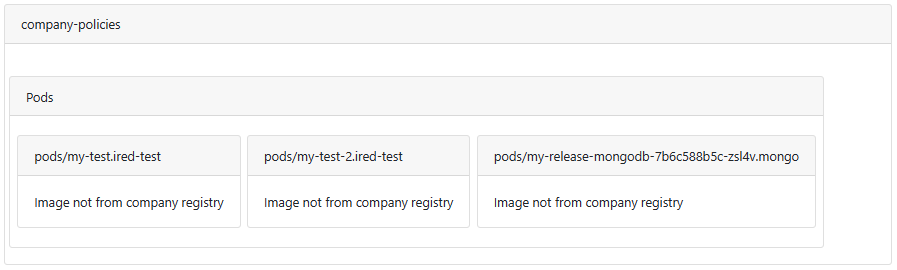
\includegraphics[width=130mm, keepaspectratio]{content/60_caseStudy2/company_policies_1.png}
  \caption{Report generated by the script}
  \label{fig:report}
\end{figure}

The report shows that there are 3 pods, which use images outside from the company registry.

Now lets do the enforcing part. Put this code inside the server block.

\begin{lstlisting}[caption={TODO},language=Kotlin,label=code:todo]
webhook("only-internal-registry") {
  operations(CREATE, UPDATE)
  apiGroups(APPS)
  apiVersions(ANY)
  resources(DEPLOYMENTS, STATEFULSETS, DAEMONSETS)
  namespaceSelector { }
  failurePolicy(FAIL)
  behavior {
    allowed {
      podSpec!!.containers.all { it.image.startsWith(companyPrefix) }
    }
    status {
      message = "All images must be from the company registry."
    }
  }
}
\end{lstlisting}

To create a rule, we need to add a `webhook` block. It needs a unique name. Lets name it "only-internal-registry". We need to define which events should the webhook listen to. In this example the webhook listens to the creation or update of any deployments, statefulsets and daemonsets.

The more interesting part is the behavior block. It describes how should the webhook behave when a request arrives. Inside the behavior block we can access the request body using many ways. One of them is the podSpec keyword. It is a shortcut to the `.spec.template.spec` of a deployment, statefulset or daemonset.

In the allowed block we can specify when to allow or reject an event. In this case we only accept events when the all the containers of the pod has an image starting with the the company prefix.

In the status block we define the error message in case the event is rejected.

Lets deploy and test our newly created agent dsl. On the monitors view we can see that the pods inside the ired-test namespace use images outside of the company registry, and the mongodb also uses an image from docker.io instead of the company registry.

We can also test that we can no longer create resources which use images outside from the company registry:

\begin{lstlisting}[caption={TODO},language=bash,label=code:bashx]
kubectl create ns policy-test
kubectl apply -f k8s/test-policy.yaml -n policy-test
\end{lstlisting}

We should get this error:

\begin{lstlisting}[caption={TODO},language=bash,label=code:todo]
Error from server: error when creating "k8s/test-policy.yaml": admission webhook "only-internal-registry.btieger.me" denied the request: All images must be from the company registry.
\end{lstlisting}

\begin{lstlisting}[caption={TODO},language=bash,label=code:bashx]
yq eval 'select(.kind == "Deployment").spec.template.spec.containers[0].image = "tiegris/apples-users"' k8s/test-policy.yaml -i
kubectl apply -f k8s/test-policy.yaml -n policy-test
\end{lstlisting}

This error shows that our rule works and is enforced.

This is the end of the demo. In this demo we saw the basic capabilities of the Konstrainer platform, some use-cases, and how to create our own rules.


\chapter{Case study 2: Creating new constraints}
\label{chap:case_study2}

The \ref{chap:case_study1} chapter only showed the capabilities of the Konstrainer framework, but did not show how to write a more advanced script, because the \nameref{chap:konst_dsl} chapter was a prerequisite for that. This chapter will continue the case study.

\section{Writing your own policies}

Let's assume the company has introduced some custom policies and, now they want to enforce them using Konstrainer. Start with a very simple policy: All images must come from the internal company registry.

To enforce this, first let's detect which pods violate this policy:

Create a file with the company-policies.kt file with the following content:

\begin{lstlisting}[caption={Report skeleton},language=Kotlin,label=code:todo]
package me.btieger

import me.btieger.dsl.*

const val companyPrefix = "tiegris/"
val companPolicies = server("company-policies") {
  report {

  }
}
\end{lstlisting}

This script has an empty report so far. As described in the \ref{sec:report} section, we should fetch the list of pods and create an aggregation group. In this case, no additional processing is needed.

\begin{lstlisting}[caption={Aggregation group},language=Kotlin,label=code:todo]
report {
  val pods = kubelist { pods() }
  aggregation("Pods", pods) {

  }
}
\end{lstlisting}

To decide if all the containers of a pod are using images only from the company registry, we must specify this requirement with mathematical precision, using first order logic. Here are two continuous sentences which, express the requirement with first order logic.

`Tag the pod, if any of its containers image does not start with the company prefix.'

`Do not tag the pod, if all of its containers image starts with the company prefix.'

\begin{lstlisting}[caption={Tag pods},language=Kotlin,label=code:todo]
report {
  aggregation("Pods", kubelist { pods() }) {
    tag("Image not from company registry") {
      item.spec.containers.any { !it.image.startsWith(companyPrefix) }
    }
  }
}
\end{lstlisting}

The script accesses the Kubernetes API, but to do that successfully, it needs authorization. We need to associate a \emph{ClusterRole} to the agent. In the demo files there is also a \emph{ClusterRole} definition. We want our agent to be least privileged, so we are only giving it read access to the pods.

\begin{lstlisting}[caption={TODO},language=Kotlin,label=code:todo]
package me.btieger
import me.btieger.dsl.*

const val companyPrefix = "tiegris/"
val companyPolicies = server("company-policies") {
  clusterRole = "read-pods"
  report {
    aggregation("Pods", kubelist { pods() }) {
      tag("Image not from company registry") {
        item.spec.containers.any { !it.image.startsWith(companyPrefix) }
      }
    }
  }
}
\end{lstlisting}

The line: `clusterRole = ReadAny` assigns the ReadAny clusterrole to the agent by creating a clusterrolebinding during the deployment of the agent. The ReadAny clusterrole is created with the Konstrainer installation, it gives read access to all resources in the cluster.

Let's test the script now. If we upload, and deploy the script, we should see it working:

\begin{figure}[h]
  \centering
  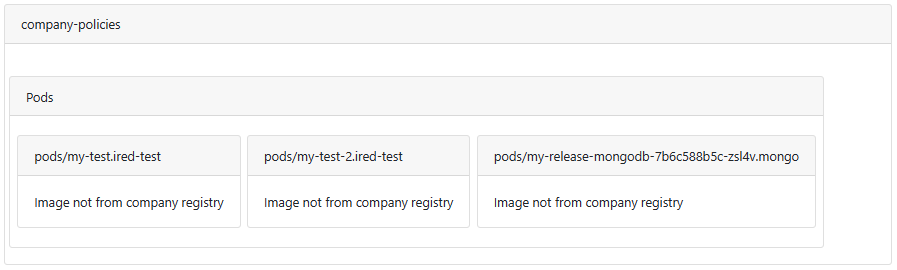
\includegraphics[width=130mm, keepaspectratio]{content/60_caseStudy2/company_policies_1.png}
  \caption{Report generated by the script}
  \label{fig:report}
\end{figure}

The report shows that there are 3 pods, which use images outside from the company registry.

Now lets do the enforcing part. Put this code inside the server block.

\begin{lstlisting}[caption={TODO},language=Kotlin,label=code:todo]
webhook("only-internal-registry") {
  operations(CREATE, UPDATE)
  apiGroups(APPS)
  apiVersions(ANY)
  resources(DEPLOYMENTS, STATEFULSETS, DAEMONSETS)
  namespaceSelector { }
  failurePolicy(FAIL)
  behavior {
    allowed {
      podSpec!!.containers.all { it.image.startsWith(companyPrefix) }
    }
    status {
      message = "All images must be from the company registry."
    }
  }
}
\end{lstlisting}

To create a rule, we need to add a `webhook` block. It needs a unique name. Lets name it "only-internal-registry". We need to define which events should the webhook listen to. In this example the webhook listens to the creation or update of any deployments, statefulsets and daemonsets.

The more interesting part is the behavior block. It describes how should the webhook behave when a request arrives. Inside the behavior block we can access the request body using many ways. One of them is the podSpec keyword. It is a shortcut to the `.spec.template.spec` of a deployment, statefulset or daemonset.

In the allowed block we can specify when to allow or reject an event. In this case we only accept events when the all the containers of the pod has an image starting with the the company prefix.

In the status block we define the error message in case the event is rejected.

Lets deploy and test our newly created agent dsl. On the monitors view we can see that the pods inside the ired-test namespace use images outside of the company registry, and the mongodb also uses an image from docker.io instead of the company registry.

We can also test that we can no longer create resources which use images outside from the company registry:

\begin{lstlisting}[caption={TODO},language=bash,label=code:bashx]
kubectl create ns policy-test
kubectl apply -f k8s/test-policy.yaml -n policy-test
\end{lstlisting}

We should get this error:

\begin{lstlisting}[caption={TODO},language=bash,label=code:todo]
Error from server: error when creating "k8s/test-policy.yaml": admission webhook "only-internal-registry.btieger.me" denied the request: All images must be from the company registry.
\end{lstlisting}

\begin{lstlisting}[caption={TODO},language=bash,label=code:bashx]
yq eval 'select(.kind == "Deployment").spec.template.spec.containers[0].image = "tiegris/apples-users"' k8s/test-policy.yaml -i
kubectl apply -f k8s/test-policy.yaml -n policy-test
\end{lstlisting}

This error shows that our rule works and is enforced.

This is the end of the demo. In this demo we saw the basic capabilities of the Konstrainer platform, some use-cases, and how to create our own rules.


\chapter{Case study 2: Creating new constraints}
\label{chap:case_study2}

The \ref{chap:case_study1} chapter only showed the capabilities of the Konstrainer framework, but did not show how to write a more advanced script, because the \nameref{chap:konst_dsl} chapter was a prerequisite for that. This chapter will continue the case study.

\section{Writing your own policies}

Let's assume the company has introduced some custom policies and, now they want to enforce them using Konstrainer. Start with a very simple policy: All images must come from the internal company registry.

To enforce this, first let's detect which pods violate this policy:

Create a file with the company-policies.kt file with the following content:

\begin{lstlisting}[caption={Report skeleton},language=Kotlin,label=code:todo]
package me.btieger

import me.btieger.dsl.*

const val companyPrefix = "tiegris/"
val companPolicies = server("company-policies") {
  report {

  }
}
\end{lstlisting}

This script has an empty report so far. As described in the \ref{sec:report} section, we should fetch the list of pods and create an aggregation group. In this case, no additional processing is needed.

\begin{lstlisting}[caption={Aggregation group},language=Kotlin,label=code:todo]
report {
  val pods = kubelist { pods() }
  aggregation("Pods", pods) {

  }
}
\end{lstlisting}

To decide if all the containers of a pod are using images only from the company registry, we must specify this requirement with mathematical precision, using first order logic. Here are two continuous sentences which, express the requirement with first order logic.

`Tag the pod, if any of its containers image does not start with the company prefix.'

`Do not tag the pod, if all of its containers image starts with the company prefix.'

\begin{lstlisting}[caption={Tag pods},language=Kotlin,label=code:todo]
report {
  aggregation("Pods", kubelist { pods() }) {
    tag("Image not from company registry") {
      item.spec.containers.any { !it.image.startsWith(companyPrefix) }
    }
  }
}
\end{lstlisting}

The script accesses the Kubernetes API, but to do that successfully, it needs authorization. We need to associate a \emph{ClusterRole} to the agent. In the demo files there is also a \emph{ClusterRole} definition. We want our agent to be least privileged, so we are only giving it read access to the pods.

\begin{lstlisting}[caption={TODO},language=Kotlin,label=code:todo]
package me.btieger
import me.btieger.dsl.*

const val companyPrefix = "tiegris/"
val companyPolicies = server("company-policies") {
  clusterRole = "read-pods"
  report {
    aggregation("Pods", kubelist { pods() }) {
      tag("Image not from company registry") {
        item.spec.containers.any { !it.image.startsWith(companyPrefix) }
      }
    }
  }
}
\end{lstlisting}

The line: `clusterRole = ReadAny` assigns the ReadAny clusterrole to the agent by creating a clusterrolebinding during the deployment of the agent. The ReadAny clusterrole is created with the Konstrainer installation, it gives read access to all resources in the cluster.

Let's test the script now. If we upload, and deploy the script, we should see it working:

\begin{figure}[h]
  \centering
  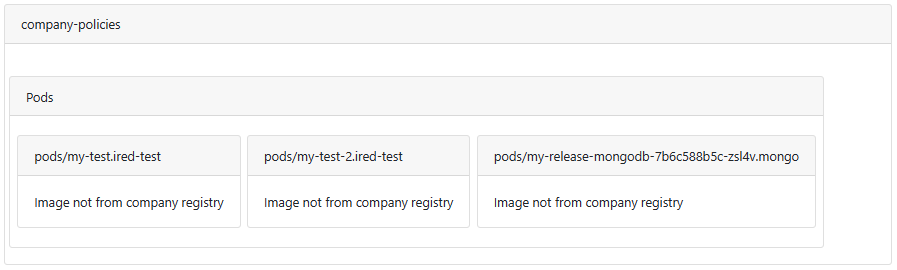
\includegraphics[width=130mm, keepaspectratio]{content/60_caseStudy2/company_policies_1.png}
  \caption{Report generated by the script}
  \label{fig:report}
\end{figure}

The report shows that there are 3 pods, which use images outside from the company registry.

Now lets do the enforcing part. Put this code inside the server block.

\begin{lstlisting}[caption={TODO},language=Kotlin,label=code:todo]
webhook("only-internal-registry") {
  operations(CREATE, UPDATE)
  apiGroups(APPS)
  apiVersions(ANY)
  resources(DEPLOYMENTS, STATEFULSETS, DAEMONSETS)
  namespaceSelector { }
  failurePolicy(FAIL)
  behavior {
    allowed {
      podSpec!!.containers.all { it.image.startsWith(companyPrefix) }
    }
    status {
      message = "All images must be from the company registry."
    }
  }
}
\end{lstlisting}

To create a rule, we need to add a `webhook` block. It needs a unique name. Lets name it "only-internal-registry". We need to define which events should the webhook listen to. In this example the webhook listens to the creation or update of any deployments, statefulsets and daemonsets.

The more interesting part is the behavior block. It describes how should the webhook behave when a request arrives. Inside the behavior block we can access the request body using many ways. One of them is the podSpec keyword. It is a shortcut to the `.spec.template.spec` of a deployment, statefulset or daemonset.

In the allowed block we can specify when to allow or reject an event. In this case we only accept events when the all the containers of the pod has an image starting with the the company prefix.

In the status block we define the error message in case the event is rejected.

Lets deploy and test our newly created agent dsl. On the monitors view we can see that the pods inside the ired-test namespace use images outside of the company registry, and the mongodb also uses an image from docker.io instead of the company registry.

We can also test that we can no longer create resources which use images outside from the company registry:

\begin{lstlisting}[caption={TODO},language=bash,label=code:bashx]
kubectl create ns policy-test
kubectl apply -f k8s/test-policy.yaml -n policy-test
\end{lstlisting}

We should get this error:

\begin{lstlisting}[caption={TODO},language=bash,label=code:todo]
Error from server: error when creating "k8s/test-policy.yaml": admission webhook "only-internal-registry.btieger.me" denied the request: All images must be from the company registry.
\end{lstlisting}

\begin{lstlisting}[caption={TODO},language=bash,label=code:bashx]
yq eval 'select(.kind == "Deployment").spec.template.spec.containers[0].image = "tiegris/apples-users"' k8s/test-policy.yaml -i
kubectl apply -f k8s/test-policy.yaml -n policy-test
\end{lstlisting}

This error shows that our rule works and is enforced.

This is the end of the demo. In this demo we saw the basic capabilities of the Konstrainer platform, some use-cases, and how to create our own rules.


% Ktor web keretrendszer: lábbal hajtós, kényelmes könnyű dinamikus koncig, kiforratlan, nincsenek best practice-ek -> konklúzió

% security

% esettanulmány: 

% dsl általánosan, ami készült <- esettanulmányon keresztül, előtte

% 

%~~~~~~~~~~~~~~~~~~~~~~~~~~~~~~~~~~~~~~~~~~~~~~~~~~~~~~~~~~~~~~~~~~~~~~~~~~~~~~~~~~~~~~


% Acknowledgements
%~~~~~~~~~~~~~~~~~~~~~~~~~~~~~~~~~~~~~~~~~~~~~~~~~~~~~~~~~~~~~~~~~~~~~~~~~~~~~~~~~~~~~~
% %----------------------------------------------------------------------------
\chapter*{\koszonetnyilvanitas}\addcontentsline{toc}{chapter}{\koszonetnyilvanitas}
%----------------------------------------------------------------------------

Szeretnék köszönetet mondani a konzulensemnek, Elekes Mártonnak az áldozatos munkájáért és segítőkészségért. Továbbá köszönöm Dr. Micskei Zoltánnak, hogy bevezette számomra SysML v2 nyelv alapjait.



% List of Figures, Tables
%~~~~~~~~~~~~~~~~~~~~~~~~~~~~~~~~~~~~~~~~~~~~~~~~~~~~~~~~~~~~~~~~~~~~~~~~~~~~~~~~~~~~~~
%\listoffigures\addcontentsline{toc}{chapter}{\listfigurename}
%\listoftables\addcontentsline{toc}{chapter}{\listtablename}


% Bibliography
%~~~~~~~~~~~~~~~~~~~~~~~~~~~~~~~~~~~~~~~~~~~~~~~~~~~~~~~~~~~~~~~~~~~~~~~~~~~~~~~~~~~~~~
\addcontentsline{toc}{chapter}{\bibname}
\bibliography{bib/mybib}


% Appendix
%~~~~~~~~~~~~~~~~~~~~~~~~~~~~~~~~~~~~~~~~~~~~~~~~~~~~~~~~~~~~~~~~~~~~~~~~~~~~~~~~~~~~~~
\chapter{Case study 2: Creating new constraints}
\label{chap:case_study2}

The \ref{chap:case_study1} chapter only showed the capabilities of the Konstrainer framework, but did not show how to write a more advanced script, because the \nameref{chap:konst_dsl} chapter was a prerequisite for that. This chapter will continue the case study.

\section{Writing your own policies}

Let's assume the company has introduced some custom policies and, now they want to enforce them using Konstrainer. Start with a very simple policy: All images must come from the internal company registry.

To enforce this, first let's detect which pods violate this policy:

Create a file with the company-policies.kt file with the following content:

\begin{lstlisting}[caption={Report skeleton},language=Kotlin,label=code:todo]
package me.btieger

import me.btieger.dsl.*

const val companyPrefix = "tiegris/"
val companPolicies = server("company-policies") {
  report {

  }
}
\end{lstlisting}

This script has an empty report so far. As described in the \ref{sec:report} section, we should fetch the list of pods and create an aggregation group. In this case, no additional processing is needed.

\begin{lstlisting}[caption={Aggregation group},language=Kotlin,label=code:todo]
report {
  val pods = kubelist { pods() }
  aggregation("Pods", pods) {

  }
}
\end{lstlisting}

To decide if all the containers of a pod are using images only from the company registry, we must specify this requirement with mathematical precision, using first order logic. Here are two continuous sentences which, express the requirement with first order logic.

`Tag the pod, if any of its containers image does not start with the company prefix.'

`Do not tag the pod, if all of its containers image starts with the company prefix.'

\begin{lstlisting}[caption={Tag pods},language=Kotlin,label=code:todo]
report {
  aggregation("Pods", kubelist { pods() }) {
    tag("Image not from company registry") {
      item.spec.containers.any { !it.image.startsWith(companyPrefix) }
    }
  }
}
\end{lstlisting}

The script accesses the Kubernetes API, but to do that successfully, it needs authorization. We need to associate a \emph{ClusterRole} to the agent. In the demo files there is also a \emph{ClusterRole} definition. We want our agent to be least privileged, so we are only giving it read access to the pods.

\begin{lstlisting}[caption={TODO},language=Kotlin,label=code:todo]
package me.btieger
import me.btieger.dsl.*

const val companyPrefix = "tiegris/"
val companyPolicies = server("company-policies") {
  clusterRole = "read-pods"
  report {
    aggregation("Pods", kubelist { pods() }) {
      tag("Image not from company registry") {
        item.spec.containers.any { !it.image.startsWith(companyPrefix) }
      }
    }
  }
}
\end{lstlisting}

The line: `clusterRole = ReadAny` assigns the ReadAny clusterrole to the agent by creating a clusterrolebinding during the deployment of the agent. The ReadAny clusterrole is created with the Konstrainer installation, it gives read access to all resources in the cluster.

Let's test the script now. If we upload, and deploy the script, we should see it working:

\begin{figure}[h]
  \centering
  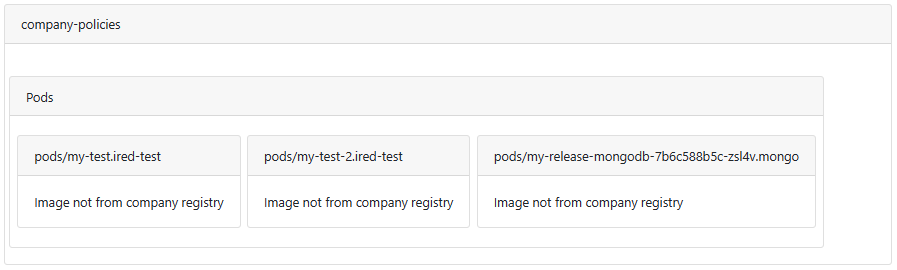
\includegraphics[width=130mm, keepaspectratio]{content/60_caseStudy2/company_policies_1.png}
  \caption{Report generated by the script}
  \label{fig:report}
\end{figure}

The report shows that there are 3 pods, which use images outside from the company registry.

Now lets do the enforcing part. Put this code inside the server block.

\begin{lstlisting}[caption={TODO},language=Kotlin,label=code:todo]
webhook("only-internal-registry") {
  operations(CREATE, UPDATE)
  apiGroups(APPS)
  apiVersions(ANY)
  resources(DEPLOYMENTS, STATEFULSETS, DAEMONSETS)
  namespaceSelector { }
  failurePolicy(FAIL)
  behavior {
    allowed {
      podSpec!!.containers.all { it.image.startsWith(companyPrefix) }
    }
    status {
      message = "All images must be from the company registry."
    }
  }
}
\end{lstlisting}

To create a rule, we need to add a `webhook` block. It needs a unique name. Lets name it "only-internal-registry". We need to define which events should the webhook listen to. In this example the webhook listens to the creation or update of any deployments, statefulsets and daemonsets.

The more interesting part is the behavior block. It describes how should the webhook behave when a request arrives. Inside the behavior block we can access the request body using many ways. One of them is the podSpec keyword. It is a shortcut to the `.spec.template.spec` of a deployment, statefulset or daemonset.

In the allowed block we can specify when to allow or reject an event. In this case we only accept events when the all the containers of the pod has an image starting with the the company prefix.

In the status block we define the error message in case the event is rejected.

Lets deploy and test our newly created agent dsl. On the monitors view we can see that the pods inside the ired-test namespace use images outside of the company registry, and the mongodb also uses an image from docker.io instead of the company registry.

We can also test that we can no longer create resources which use images outside from the company registry:

\begin{lstlisting}[caption={TODO},language=bash,label=code:bashx]
kubectl create ns policy-test
kubectl apply -f k8s/test-policy.yaml -n policy-test
\end{lstlisting}

We should get this error:

\begin{lstlisting}[caption={TODO},language=bash,label=code:todo]
Error from server: error when creating "k8s/test-policy.yaml": admission webhook "only-internal-registry.btieger.me" denied the request: All images must be from the company registry.
\end{lstlisting}

\begin{lstlisting}[caption={TODO},language=bash,label=code:bashx]
yq eval 'select(.kind == "Deployment").spec.template.spec.containers[0].image = "tiegris/apples-users"' k8s/test-policy.yaml -i
kubectl apply -f k8s/test-policy.yaml -n policy-test
\end{lstlisting}

This error shows that our rule works and is enforced.

This is the end of the demo. In this demo we saw the basic capabilities of the Konstrainer platform, some use-cases, and how to create our own rules.


%\label{page:last}
\end{document}
